% Options for packages loaded elsewhere
\PassOptionsToPackage{unicode}{hyperref}
\PassOptionsToPackage{hyphens}{url}
%
\documentclass[
]{article}
\usepackage{lmodern}
\usepackage{amssymb,amsmath}
\usepackage{ifxetex,ifluatex}
\ifnum 0\ifxetex 1\fi\ifluatex 1\fi=0 % if pdftex
  \usepackage[T1]{fontenc}
  \usepackage[utf8]{inputenc}
  \usepackage{textcomp} % provide euro and other symbols
\else % if luatex or xetex
  \usepackage{unicode-math}
  \defaultfontfeatures{Scale=MatchLowercase}
  \defaultfontfeatures[\rmfamily]{Ligatures=TeX,Scale=1}
\fi
% Use upquote if available, for straight quotes in verbatim environments
\IfFileExists{upquote.sty}{\usepackage{upquote}}{}
\IfFileExists{microtype.sty}{% use microtype if available
  \usepackage[]{microtype}
  \UseMicrotypeSet[protrusion]{basicmath} % disable protrusion for tt fonts
}{}
\makeatletter
\@ifundefined{KOMAClassName}{% if non-KOMA class
  \IfFileExists{parskip.sty}{%
    \usepackage{parskip}
  }{% else
    \setlength{\parindent}{0pt}
    \setlength{\parskip}{6pt plus 2pt minus 1pt}}
}{% if KOMA class
  \KOMAoptions{parskip=half}}
\makeatother
\usepackage{xcolor}
\IfFileExists{xurl.sty}{\usepackage{xurl}}{} % add URL line breaks if available
\IfFileExists{bookmark.sty}{\usepackage{bookmark}}{\usepackage{hyperref}}
\hypersetup{
  pdftitle={Annotated Bibliography},
  pdfauthor={Nate Lant},
  hidelinks,
  pdfcreator={LaTeX via pandoc}}
\urlstyle{same} % disable monospaced font for URLs
\usepackage[margin=1in]{geometry}
\usepackage{graphicx,grffile}
\makeatletter
\def\maxwidth{\ifdim\Gin@nat@width>\linewidth\linewidth\else\Gin@nat@width\fi}
\def\maxheight{\ifdim\Gin@nat@height>\textheight\textheight\else\Gin@nat@height\fi}
\makeatother
% Scale images if necessary, so that they will not overflow the page
% margins by default, and it is still possible to overwrite the defaults
% using explicit options in \includegraphics[width, height, ...]{}
\setkeys{Gin}{width=\maxwidth,height=\maxheight,keepaspectratio}
% Set default figure placement to htbp
\makeatletter
\def\fps@figure{htbp}
\makeatother
\setlength{\emergencystretch}{3em} % prevent overfull lines
\providecommand{\tightlist}{%
  \setlength{\itemsep}{0pt}\setlength{\parskip}{0pt}}
\setcounter{secnumdepth}{-\maxdimen} % remove section numbering

\title{Annotated Bibliography}
\author{Nate Lant}
\date{}

\begin{document}
\maketitle

\hypertarget{microsimulation}{%
\section{Microsimulation}\label{microsimulation}}

Buzz words: multi-agent, microsimulation model, on-demand, agent-based,
carpooling, travel demand/supply estimation, taxi fleets,
demand-responsive transportation, case study,

\hypertarget{autonomous-taxicabs-in-berlin-a-spatiotemporal-analysis-of-service-performance}{%
\subsection{Autonomous Taxicabs in Berlin -- A Spatiotemporal Analysis
of Service
Performance}\label{autonomous-taxicabs-in-berlin-a-spatiotemporal-analysis-of-service-performance}}

Bischoff J, Maciejewski M (2016). ``Autonomous Taxicabs in Berlin â€``
A, Spatiotemporal Analysis of Service Performance.''
\emph{Transportation, Research Procedia}, \emph{19}, 176-186. ISSN
23521465, doi:, 10.1016/j.trpro.2016.12.078 (URL:,
\url{https://doi.org/10.1016/j.trpro.2016.12.078}), \textless URL:,
www.sciencedirect.com,
\url{https://linkinghub.elsevier.com/retrieve/pii/S235214651630864X}\textgreater.

\hypertarget{abstract}{%
\subsubsection{Abstract}\label{abstract}}

\hypertarget{notes}{%
\subsubsection{Notes}\label{notes}}

They tested the effect on traffic from empty cars and demand shift as
people switch from public transit.

They show how they scale from the 100\% base scenario to the 10\%
without describing how they scaled down trip rates and network capacity
(maybe described in previous paper).

Helpful graphics include the passenger waiting times during time of day,
the productivity of the vehicles during time of day, and spatial
distribution of waiting times and empty rides.

They found 10\% of transit riders switched to autonomous taxis (only
measured on the city center model, no outskirts). No explanation was
given.

\hypertarget{simulation-of-city-wide-replacement-of-private-cars-with-autonomous-taxis-in-berlin}{%
\subsection{Simulation of city-wide replacement of private cars with
autonomous taxis in
Berlin}\label{simulation-of-city-wide-replacement-of-private-cars-with-autonomous-taxis-in-berlin}}

Bischoff J, Maciejewski M (2016). ``ScienceDirect Simulation of,
city-wide replacement of private cars with autonomous taxis in
Berlin.'', \emph{Procedia Computer Science}, \emph{83}, 237-244. doi:,
10.1016/j.procs.2016.04.121 (URL:,
\url{https://doi.org/10.1016/j.procs.2016.04.121}), \textless URL:,
www.sciencedirect.com\textgreater.

\hypertarget{abstract-1}{%
\subsubsection{Abstract}\label{abstract-1}}

\hypertarget{notes-1}{%
\subsubsection{Notes}\label{notes-1}}

Goal is to find optimum number of autonomous taxis (ATs) to service the
city of Berlin, by replacing the private cars. They came up with 100,000
(not sure how exactly)

Details include the dispatching strategy using the demand-supply
balancing strategy, \emph{undersupply} and \emph{oversupply}.

I think the dispatch algorithm should include a buffer distance around
the request. The model should be seen from the customer's perspective.

Data not supported\ldots{} - The split of car and public transit. -
Section 3.2, certain adaptations pertaining to shortest path
search\ldots{} - What are taxi ranks (section 4) - 4.2, the graphs all
look the same, and they don't talk about why 100,000 vehicles were
chosen. ``It was a good compromise\ldots{}'' - 4.3 the Replacement
ratio\ldots{} is it 1:10 or 1:12? - 4.3.2 where did they get the 40 min
utilization of CDVs? - Conclusion, total drive time? what is it?

\hypertarget{simulating-a-rich-ride-share-mobility-service-using-agent-based-models}{%
\subsection{Simulating a rich ride-share mobility service using
agent-based
models}\label{simulating-a-rich-ride-share-mobility-service-using-agent-based-models}}

Segui-Gasco P, Ballis H, Parisi V, Kelsall DG, North RJ, Busquets D,
(2019). ``Simulating a rich ride-share mobility service using,
agent-based models.'' \emph{Transportation}. ISSN 0049-4488, doi:,
10.1007/s11116-019-10012-y (URL:,
\url{https://doi.org/10.1007/s11116-019-10012-y}).

\hypertarget{abstract-2}{%
\subsubsection{Abstract}\label{abstract-2}}

In the UK, and using the National Trip End Model (NTEM), they produced a
set of O-D matrices and then integrated them into MATSim. MATSim was
used to predict the changes in travel behavior (specifically mode shift)
and predict the effect on traffic conditions due to new AMoD services
for the year 2025. As part of their agent-based framework, the Value of
Time changes depending on the purpose of each trips and the income of
the traveler.

MATSim is used to calculate the service demand, however, neither the
occupancy of each vehicle and waiting/detour time were known. Average
values were used and held constant (IMSim could have precisely
calculated those values, but it would have taken a lot of time\ldots).

MATSim informs the IMSim about the network conditions (travel times) and
origins and destinations. With this input, IMSims calculates the optimum
routes for the AMoD fleet, while simultaneously tracking the waiting and
detour times that each agent experiences. ``This information'' (not
exactly sure what is included here) is reported back to MATSim which
updates the perception score of the agents and the Passenger Car Unit
factor.

Then they calibrate it to the MERGE Greenwich case study in London.

\hypertarget{notes-2}{%
\subsubsection{Notes}\label{notes-2}}

In London, using MATSim (demand simulation model) coupled with IMSim
(Intelligent mobility simulator)

Includes a literature review that describes several authors' efforts.

OD trips had to be disaggregated? What does that mean? Each trip was
assigned information regarding the purpose, departure time, and initial
mode of transport before the introduction of AV ride-sharing. The Value
of Time (VoT) for each trip was also included together with demographic
characteristics.

the original transport demand derives from a trip-based model, no
information can be extracted regarding the sequence of activities
(trip-chaining). Instead, all plans were expressed as two activities:
one at the origin and one at the destination, linked by an intermediate
trip.

\hypertarget{microsimulation-of-demand-and-supply-of-autonomous-mobility-on-demand}{%
\subsection{Microsimulation of Demand and Supply of Autonomous Mobility
On
Demand}\label{microsimulation-of-demand-and-supply-of-autonomous-mobility-on-demand}}

Azevedo CL, Marczuk K, Raveau S, Soh H, Adnan M, Basak K, Loganathan H,,
Deshmunkh N, Lee DH, Frazzoli E, Ben-Akiva M (2016). ``Microsimulation,
of demand and supply of autonomous mobility on demand.''
\emph{Transportation, Research Record}, \emph{2564}, 21-30. ISSN
03611981, doi: 10.3141/2564-03, (URL:
\url{https://doi.org/10.3141/2564-03}).

\hypertarget{abstract-3}{%
\subsubsection{Abstract}\label{abstract-3}}

Using SimMobility, they integrate mobility sensitive behavioral models
in a multiple time-scale structure. They look at three simulation levels
a) long-term, b) a midterm level, and c) a short-term level.

\hypertarget{notes-3}{%
\subsubsection{Notes}\label{notes-3}}

Professors from the MIT-Singapore alliance.

\hypertarget{taxisim-a-multiagent-simulation-platform-for-evaluating-taxi-fleet-operations}{%
\subsection{TaxiSim: A Multiagent Simulation Platform for Evaluating
Taxi Fleet
Operations}\label{taxisim-a-multiagent-simulation-platform-for-evaluating-taxi-fleet-operations}}

Cheng S, Nguyen TD (2011). ``TaxiSim: A Multiagent Simulation Platform,
for Evaluating Taxi Fleet Operations.'' In \emph{2011 IEEE/WIC/ACM,
International Conferences on Web Intelligence and Intelligent Agent,
Technology}, 14-21. ISBN 978-1-4577-1373-6, doi:,
10.1109/WI-IAT.2011.138 (URL:
\url{https://doi.org/10.1109/WI-IAT.2011.138}),, \textless URL:
\url{http://ieeexplore.ieee.org/document/6040748/}\textgreater.

\hypertarget{abstract-4}{%
\subsubsection{Abstract}\label{abstract-4}}

They \emph{build} a multi-agent-base simulation platform, TaxiSim.

\hypertarget{notes-4}{%
\subsubsection{Notes}\label{notes-4}}

``Despite all these efforts in building computer simulations for a wide
range of studies, to the best of our knowledge, we cannot find any
simulation platform that is capable of modeling realistic taxi fleet
operations. Taxi fleet operation is special and cannot be modeled
straightforwardly by using existing technologies for the following
reasons: {[}Taxi drivers make decisions "selfishly" and taxi drivers act
unpredictably after they drop off a customer.{]}''

\hypertarget{output-variability-caused-by-random-seeds-in-a-multi-agent-transport-simulation-model}{%
\subsection{Output variability caused by random seeds in a multi-agent
transport simulation
model}\label{output-variability-caused-by-random-seeds-in-a-multi-agent-transport-simulation-model}}

Paulsen M, Rasmussen TK, Nielsen OA (2018). ``Output variability caused,
by random seeds in a multi-agent transport simulation model.'' In,
\emph{Procedia Computer Science}, volume 130, 850-857. doi:,
10.1016/j.procs.2018.04.078 (URL:,
\url{https://doi.org/10.1016/j.procs.2018.04.078}).

\hypertarget{abstract-5}{%
\subsubsection{Abstract}\label{abstract-5}}

In this study they analyse the output variability caused by random seeds
of a multi-agent transport simulator (MATSim) when applied to a case
study of Santiago, Chile.

\hypertarget{notes-5}{%
\subsubsection{Notes}\label{notes-5}}

\hypertarget{a-critical-analysis-of-travel-demand-estimation-for-new-one-way-carsharing-systems}{%
\subsection{A Critical Analysis of Travel Demand Estimation for New
One-Way Carsharing
Systems}\label{a-critical-analysis-of-travel-demand-estimation-for-new-one-way-carsharing-systems}}

\hypertarget{abstract-6}{%
\subsubsection{Abstract}\label{abstract-6}}

This paper discusses the methods, paradigms, toolkits and platforms used
by other researchers for the demand estimation of one-way carsharing
systems. It is a collection of information.

\hypertarget{notes-6}{%
\subsubsection{Notes}\label{notes-6}}

Probably more helpful to learn from than to cite.

Includes an informative table with summary of studies on travel demand
estimation for one-way carsharing systems (includes Axhausen, Ciari,
Balac, Fagnant, and Horl - all using MATSim)

\hypertarget{an-assignment-based-approach-to-efficient-real-time-city-scale-taxi-dispatching}{%
\subsection{An Assignment-Based Approach to Efficient Real-Time
City-Scale Taxi
Dispatching}\label{an-assignment-based-approach-to-efficient-real-time-city-scale-taxi-dispatching}}

Maciejewski M, Bischoff J, Nagel K (2016). ``An Assignment-Based,
Approach to Efficient Real-Time City-Scale Taxi Dispatching.''
\emph{IEEE, Intelligent Systems}, \emph{31}(1), 68-77. ISSN 15411672,
doi:, 10.1109/MIS.2016.2 (URL:
\url{https://doi.org/10.1109/MIS.2016.2}).

\hypertarget{abstract-7}{%
\subsubsection{Abstract}\label{abstract-7}}

\hypertarget{notes-7}{%
\subsubsection{Notes}\label{notes-7}}

They evaluate dispatching strategies in detail in the city of Berlin and
the neighboring region of Brandenburg using the microscopic large-scale
MATSim simulator.

\hypertarget{carsharing-demand-estimation-zurich-switzerland-area-case-study}{%
\subsection{Carsharing demand estimation Zurich, Switzerland, area case
study}\label{carsharing-demand-estimation-zurich-switzerland-area-case-study}}

\hypertarget{abstract-8}{%
\subsubsection{Abstract}\label{abstract-8}}

\hypertarget{notes-8}{%
\subsubsection{Notes}\label{notes-8}}

\hypertarget{the-philippines-agent-based-transport-simulation-model-for-disaster-response-vehicles}{%
\subsection{The Philippines: Agent-Based Transport Simulation Model for
Disaster Response
Vehicles}\label{the-philippines-agent-based-transport-simulation-model-for-disaster-response-vehicles}}

Yaneza EB (2016). ``The Philippines: Agent-Based Transport Simulation,
Model for Disaster Response Vehicles.'' In \emph{The Multi-Agent
Transport, Simulation MATSim}, 461-468. Ubiquity Press. doi:
10.5334/baw.78 (URL:, \url{https://doi.org/10.5334/baw.78}),
\textless URL:,
\url{http://www.ubiquitypress.com/site/chapters/10.5334/baw.78/}\textgreater.

\hypertarget{abstract-9}{%
\subsubsection{Abstract}\label{abstract-9}}

\hypertarget{notes-9}{%
\subsubsection{Notes}\label{notes-9}}

\hypertarget{using-passive-data-to-build-an-agile-tour-based-model-a-case-study-in-asheville}{%
\subsection{USING PASSIVE DATA TO BUILD AN AGILE TOUR-BASED MODEL: A
CASE STUDY IN
ASHEVILLE}\label{using-passive-data-to-build-an-agile-tour-based-model-a-case-study-in-asheville}}

\hypertarget{abstract-10}{%
\subsubsection{Abstract}\label{abstract-10}}

\hypertarget{notes-10}{%
\subsubsection{Notes}\label{notes-10}}

\hypertarget{validating-and-calibrating-agent-based-models-a-case-study}{%
\subsection{Validating and calibrating agent-based models: A case
study}\label{validating-and-calibrating-agent-based-models-a-case-study}}

Bianchi C, Cirillo P, Gallegati M, Vagliasindi PA (2007). ``Validating,
and calibrating agent-based models: A case study.'' \emph{Computational,
Economics}, \emph{30}(3), 245-264. ISSN 09277099, doi:,
10.1007/s10614-007-9097-z (URL:,
\url{https://doi.org/10.1007/s10614-007-9097-z}).

\hypertarget{abstract-11}{%
\subsubsection{Abstract}\label{abstract-11}}

\hypertarget{notes-11}{%
\subsubsection{Notes}\label{notes-11}}

What are ad hoc perameter values?

Uses the complex adaptive trivial system (CATS) model - this means

Italian professors (various universities). There are some grammatical
errors.

\hypertarget{multi-agent-simulation-for-planning-and-designing-new-shared-mobility-services}{%
\subsection{Multi-agent simulation for planning and designing new shared
mobility
services}\label{multi-agent-simulation-for-planning-and-designing-new-shared-mobility-services}}

Inturri G, Le Pira M, Giuffrida N, Ignaccolo M, Pluchino A, Rapisarda,
A, D'Angelo R (2019). ``Multi-agent simulation for planning and,
designing new shared mobility services.'' \emph{Research in
Transportation, Economics}, \emph{73}, 34-44. ISSN 07398859, doi:,
10.1016/j.retrec.2018.11.009 (URL:,
\url{https://doi.org/10.1016/j.retrec.2018.11.009}).

\hypertarget{abstract-12}{%
\subsubsection{Abstract}\label{abstract-12}}

They use an agent-based model to explore different system configurations
of flexible transit (a specific demand responsive shared transport
service) to estimate demand and supply in the city of Ragusa, Italy.
They aim to use GIS based demand and road network models, explore
dispatching strategies, find indicators to monitor efficiency. They
identify an optimal range of operational vehicles.

\hypertarget{notes-12}{%
\subsubsection{Notes}\label{notes-12}}

\hypertarget{agent-based-simulation-testbed-for-on-demand-mobility-services}{%
\subsection{Agent-based simulation testbed for on-demand mobility
services}\label{agent-based-simulation-testbed-for-on-demand-mobility-services}}

Certick'y M, Jakob M, P'ibil R, Moler Z (2014). ``Agent-based,
simulation testbed for on-demand mobility services.'' In \emph{Procedia,
Computer Science}, volume 32, 808-815. doi: 10.1016/j.procs.2014.05.495,
(URL: \url{https://doi.org/10.1016/j.procs.2014.05.495}).

\hypertarget{abstract-13}{%
\subsubsection{Abstract}\label{abstract-13}}

\hypertarget{notes-13}{%
\subsubsection{Notes}\label{notes-13}}

The simulation testbed is built on the versatile transport simulation
framework AgentPolis.

\hypertarget{effects-of-scaling-down-the-population-for-agent-based-traffic-simulations}{%
\subsection{Effects of scaling down the population for agent-based
traffic
simulations}\label{effects-of-scaling-down-the-population-for-agent-based-traffic-simulations}}

Llorca C, Moeckel R (2019). ``Effects of scaling down the population
for, agent-based traffic simulations.'' \emph{Procedia Computer
Science}, \emph{151},, 782-787. ISSN 18770509, doi:
10.1016/j.procs.2019.04.106 (URL:,
\url{https://doi.org/10.1016/j.procs.2019.04.106}).

\hypertarget{abstract-14}{%
\subsubsection{Abstract}\label{abstract-14}}

Scaling down large populations is required because of runtime. In Munich
5\% of agents and 50 iterations produced similar travel time
distributions to the 100\% of agents and 500 iterations (but 50 times
faster). The researchers compared runtime, average travel time, and
travel time distribution.

\hypertarget{notes-14}{%
\subsubsection{Notes}\label{notes-14}}

Using MATSim and carried out in the Munich metropolitan area.

\hypertarget{heterogeneous-tolls-and-values-of-time-in-multi-agent-transport-simulation}{%
\subsection{Heterogeneous tolls and values of time in multi-agent
transport
simulation}\label{heterogeneous-tolls-and-values-of-time-in-multi-agent-transport-simulation}}

Nagel K, Kickhöfer B, Joubert JW (2014). ``Heterogeneous tolls and,
values of time in multi-agent transport simulation.'' In \emph{Procedia,
Computer Science}, volume 32, 762-768. doi: 10.1016/j.procs.2014.05.488,
(URL: \url{https://doi.org/10.1016/j.procs.2014.05.488}).

\hypertarget{abstract-15}{%
\subsubsection{Abstract}\label{abstract-15}}

\hypertarget{notes-15}{%
\subsubsection{Notes}\label{notes-15}}

\hypertarget{simulating-ad-hoc-demand-responsive-transportation-a-comparison-of-three-approaches}{%
\subsection{Simulating ad-hoc demand-responsive transportation: a
comparison of three
approaches}\label{simulating-ad-hoc-demand-responsive-transportation-a-comparison-of-three-approaches}}

Ronald N, Thompson R, Winter S (2017). ``Simulating ad-hoc,
demand-responsive transportation: a comparison of three approaches.'',
\emph{Transportation Planning and Technology}, \emph{40}(3), 340-358.
ISSN, 10290354, doi: 10.1080/03081060.2017.1283159 (URL:,
\url{https://doi.org/10.1080/03081060.2017.1283159}).

\hypertarget{abstract-16}{%
\subsubsection{Abstract}\label{abstract-16}}

The three approaches are 1) a simple custom-developed package, 2)
traffic microsimulation, and 3) agent-based simulation. Each approach is
used to analyze the advantages and disadvantages in evaluating for
demand-responsive transportation.

\hypertarget{notes-16}{%
\subsubsection{Notes}\label{notes-16}}

Researchers from University of Melbourne

\hypertarget{dynamic-ride-sharing-and-fleet-sizing-for-a-system-of-shared-1-autonomous-vehicles-in-austin-texas-2-3-4}{%
\subsection{DYNAMIC RIDE-SHARING AND FLEET SIZING FOR A SYSTEM OF SHARED
1 AUTONOMOUS VEHICLES IN AUSTIN, TEXAS 2 3
4}\label{dynamic-ride-sharing-and-fleet-sizing-for-a-system-of-shared-1-autonomous-vehicles-in-austin-texas-2-3-4}}

\hypertarget{abstract-17}{%
\subsubsection{Abstract}\label{abstract-17}}

\hypertarget{notes-17}{%
\subsubsection{Notes}\label{notes-17}}

\hypertarget{simulating-demand-responsive-transportation-a-review-of-agent-based-approaches}{%
\subsection{Simulating Demand-responsive Transportation: A Review of
Agent-based
Approaches}\label{simulating-demand-responsive-transportation-a-review-of-agent-based-approaches}}

Ronald N, Thompson R, Winter S (2015). ``Simulating Demand-responsive,
Transportation: A Review of Agent-based Approaches.'' \emph{Transport,
Reviews}, \emph{35}(4), 404-421. ISSN 14645327, doi:,
10.1080/01441647.2015.1017749 (URL:,
\url{https://doi.org/10.1080/01441647.2015.1017749}).

\hypertarget{abstract-18}{%
\subsubsection{Abstract}\label{abstract-18}}

\hypertarget{notes-18}{%
\subsubsection{Notes}\label{notes-18}}

\hypertarget{a-conceptual-design-of-an-agent-based-interaction-model-for-the-carpooling-application}{%
\subsection{A Conceptual Design of an Agent-based Interaction Model for
the Carpooling
Application}\label{a-conceptual-design-of-an-agent-based-interaction-model-for-the-carpooling-application}}

Cho S, Yasar AUH, Knapen L, Bellemans T, Janssens D, Wets G (2012). ``A,
Conceptual Design of an Agent-based Interaction Model for the,
Carpooling Application.'' In \emph{Procedia Computer Science}, volume
10,, 801-807. doi: 10.1016/j.procs.2012.06.103 (URL:,
\url{https://doi.org/10.1016/j.procs.2012.06.103}).

\hypertarget{abstract-19}{%
\subsubsection{Abstract}\label{abstract-19}}

\hypertarget{notes-19}{%
\subsubsection{Notes}\label{notes-19}}

(PDF is linked to a dial-a-ride paper by Fu)

\hypertarget{simulation-model-of-carpooling-with-the-janus-multiagent-platform}{%
\subsection{Simulation model of carpooling with the Janus Multiagent
platform}\label{simulation-model-of-carpooling-with-the-janus-multiagent-platform}}

Galland S, Gaud N, Yasar AUH, Knapen L, Janssens D, Lamotte O (2013).,
``Simulation model of carpooling with the Janus Multiagent platform.''
In, \emph{Procedia Computer Science}, volume 19, 860-866. doi:,
10.1016/j.procs.2013.06.115 (URL:,
\url{https://doi.org/10.1016/j.procs.2013.06.115}).

\hypertarget{abstract-20}{%
\subsubsection{Abstract}\label{abstract-20}}

\hypertarget{notes-20}{%
\subsubsection{Notes}\label{notes-20}}

\hypertarget{a-modeling-system-for-simulation-of-dial-a-ride-services}{%
\subsection{A modeling system for simulation of dial-a-ride
services}\label{a-modeling-system-for-simulation-of-dial-a-ride-services}}

Häll CH, Högberg M, Lundgren JT (2012). ``A modeling system for,
simulation of dial-a-ride services.'' \emph{Public Transport},
\emph{4}(1), 17-37., ISSN 1866749X, doi: 10.1007/s12469-012-0052-6
(URL:, \url{https://doi.org/10.1007/s12469-012-0052-6}).

\hypertarget{abstract-21}{%
\subsubsection{Abstract}\label{abstract-21}}

\hypertarget{notes-21}{%
\subsubsection{Notes}\label{notes-21}}

\hypertarget{estimating-activity-and-health-impacts-of-first-and-last-mile-transit-access-programs-for-work-and}{%
\subsection{Estimating Activity and Health Impacts of First and Last
Mile Transit Access Programs for Work
and}\label{estimating-activity-and-health-impacts-of-first-and-last-mile-transit-access-programs-for-work-and}}

\hypertarget{shopping-trips-using-sharing-mobility-services-in-the-metropolitan-area-center-for-transportation}{%
\subsection{Shopping Trips Using Sharing Mobility Services in the
Metropolitan Area Center for
Transportation,}\label{shopping-trips-using-sharing-mobility-services-in-the-metropolitan-area-center-for-transportation}}

\hypertarget{environment-and-community-health-final-report}{%
\subsection{Environment, and Community Health Final
Report}\label{environment-and-community-health-final-report}}

\hypertarget{abstract-22}{%
\subsubsection{Abstract}\label{abstract-22}}

\hypertarget{notes-22}{%
\subsubsection{Notes}\label{notes-22}}

\hypertarget{dynamic-transport-services}{%
\subsection{Dynamic Transport
Services}\label{dynamic-transport-services}}

Axhausen K, Nagel K, Horni A (eds.) (2016). \emph{Multi-Agent Transport,
Simulation MATSim}. Ubiquity Press, London. ISBN 978-1-909188-75-4,,
978-1-909188-76-1, 978-1-909188-77-8, 978-1-909188-78-5, doi:,
10.5334/baw (URL: \url{https://doi.org/10.5334/baw}).

\hypertarget{abstract-23}{%
\subsubsection{Abstract}\label{abstract-23}}

\hypertarget{notes-23}{%
\subsubsection{Notes}\label{notes-23}}

\hypertarget{large-scale-agent-based-transport-simulation-in-shanghai-china}{%
\subsection{Large-scale agent-based transport simulation in shanghai,
china}\label{large-scale-agent-based-transport-simulation-in-shanghai-china}}

Zhang L, Yang W, Wang J, Rao Q (2013). ``Large-scale agent-based,
transport simulation in shanghai, china.'' \emph{Transportation
Research, Record}, 34-43. ISSN 03611981, doi: 10.3141/2399-04 (URL:,
\url{https://doi.org/10.3141/2399-04}).

\hypertarget{abstract-24}{%
\subsubsection{Abstract}\label{abstract-24}}

\hypertarget{notes-24}{%
\subsubsection{Notes}\label{notes-24}}

\hypertarget{the-matsim-open-berlin-scenario-a-multimodal-agent-based-transport-simulation-scenario-based-on}{%
\subsection{The MATSim Open Berlin Scenario: A multimodal agent-based
transport simulation scenario based
on}\label{the-matsim-open-berlin-scenario-a-multimodal-agent-based-transport-simulation-scenario-based-on}}

\hypertarget{synthetic-demand-modeling-and-open-data}{%
\subsection{synthetic demand modeling and open
data}\label{synthetic-demand-modeling-and-open-data}}

Ziemke D, Kaddoura I, Nagel K (2019). ``The MATSim Open Berlin
Scenario:, A multimodal agent-based transport simulation scenario based
on, synthetic demand modeling and open data.'' \emph{Procedia Computer
Science},, \emph{151}, 870-877. ISSN 18770509, doi:
10.1016/j.procs.2019.04.120 (URL:,
\url{https://doi.org/10.1016/j.procs.2019.04.120}).

\hypertarget{abstract-25}{%
\subsubsection{Abstract}\label{abstract-25}}

\hypertarget{notes-25}{%
\subsubsection{Notes}\label{notes-25}}

\hypertarget{mobility-for-the-disabled}{%
\section{Mobility for the Disabled}\label{mobility-for-the-disabled}}

Buzz words:

\hypertarget{tncs-and-disbled-access---sfmta}{%
\subsection{TNCs and Disbled Access -
SFMTA}\label{tncs-and-disbled-access---sfmta}}

\hypertarget{california-sb-1376}{%
\subsection{California SB 1376}\label{california-sb-1376}}

\hypertarget{abstract-26}{%
\subsubsection{Abstract}\label{abstract-26}}

In September of 2018, the State of California filed SB 1376 which
``requires the Public Utilities Commission, by January 1, 2019, to begin
conducting workshops with stakeholders in order to determine community
WAV demand and WAV supply and to develop and provide recommendations
regarding specified topics for programs for on-demand services and
partnerships. The bill would require each TNC, by July 1, 2019, to pay
on a quarterly basis to the commission an amount equivalent to, at a
minimum, \$0.05 for each TNC trip completed. The bill would require
moneys collected by the commission to be deposited in the TNC Access for
All Fund, which the bill would create, and would continuously
appropriate moneys deposited in the fund to the commission for purposes
of the program. The bill would require the commission to distribute
funds from the TNC Access for All Fund on a competitive basis to access
providers that establish on-demand transportation programs or
partnerships to meet the needs of persons with disabilities.''

\hypertarget{new-york-state-transportation-newtork-company-accessibility-task-force}{%
\subsection{New York State Transportation Newtork Company Accessibility
Task
Force}\label{new-york-state-transportation-newtork-company-accessibility-task-force}}

\hypertarget{notes-26}{%
\subsubsection{Notes}\label{notes-26}}

In 2018, the Taxi and Limousine Commission (TLC) in New York City issued
a mandate requiring Uber, Lyft and Via to make wheelchair accessible
service a growing part of their operations. While this particular
mandate was not adopted, a settlement was reached in the New York State
Supreme Court. The NYC TLC retained the mandate that would require
\ldots{} TNCs to meet a wait-time requirement. The wait time requirement
states that, by 2021, TNCs must either service at least 80 percent of
requests for wheelchair-accessible vehicles in under 10 minutes and 90
percent in under 15 minutes, or associate with a company that has the
capacity to meet those requirements ().

\hypertarget{travel-patterns-of-american-adults-with-disabilities}{%
\subsection{Travel Patterns of American Adults with
Disabilities}\label{travel-patterns-of-american-adults-with-disabilities}}

\hypertarget{abstract-27}{%
\subsubsection{Abstract}\label{abstract-27}}

This paper briefly covers employment, vehicle ownership, trip purpose,
mode choice, trip distance, travel times, trip substitutes,

\hypertarget{notes-27}{%
\subsubsection{Notes}\label{notes-27}}

The NHTS asks respondents if they have ``a temporary or permanent
condition or handicap that makes it difficult to travel outside of the
home.'' If they respond yes, the NHTS asks followup questions about the
mobility devices they use, such as canes or wheelchairs. It also asks
follow-up questions about how the condition affects their travel---for
example, by limiting their driving to daytime. Some respondents have
disabilities that might not limit travel, but the NHTS asks only about
``travel- limiting disabilities.''

Over half (57.8 percent) of all respondents with disabilities use one or
more medical devices:

Walking canes (36.7 percent) Walkers (22.9 percent) Wheelchairs (11.6
percent) Motorized scooters (4.4 percent) Motorized wheelchairs (3.9
percent) Crutches (2.6 percent) White canes for visual impairments (1.3
percent) Seeing-eye dogs (1.1 percent)

Over one-third (36.5 percent) of people with disabilities who made zero
trips say that they stayed home because they have disabilities or are
housebound.

Most ride-hailing services use applications on smartphones or tablets.
People with disabilities use these devices less often than people
without disabilities. Over four-fifths (86.5 percent) of people without
disabilities use a smartphone daily versus 66.5 percent for people with
disabilities.

\hypertarget{the-impacts-of-limited-transportation-access-on-persons-with-disabilities-social-participation}{%
\subsection{The impacts of limited transportation access on persons with
disabilities' social
participation}\label{the-impacts-of-limited-transportation-access-on-persons-with-disabilities-social-participation}}

Bascom GW, Christensen KM (2017). ``The impacts of limited,
transportation access on persons with disabilities' social,
participation.'' \emph{Journal of Transport \& Health}, \emph{7},
227-234. ISSN, 2214-1405, doi: 10.1016/J.JTH.2017.10.002 (URL:,
\url{https://doi.org/10.1016/J.JTH.2017.10.002}), \textless URL:,
\url{https://www.sciencedirect.com/science/article/pii/S2214140517300075}\textgreater.

\hypertarget{abstract-28}{%
\subsubsection{Abstract}\label{abstract-28}}

\hypertarget{notes-28}{%
\subsubsection{Notes}\label{notes-28}}

(Graydon W. Bascom, Keith M. Christensen) The overall goal of the
research was to see how social life was impacted by limited
transportation because of a disability. They looked at the strength of
the social network of each individual. They also looked at what modes
were being used and if modes were associated with age, gender, race,
income, employment, type of disability, and education.

Nearly 70\% of individuals with disabilities reported that their social
life was hindered by transportation needs. And social networks affected
mode choice.

\hypertarget{demographics}{%
\subparagraph{Demographics}\label{demographics}}

Results seem slightly different from the NHTS research that I did.
According to their survey (they also included 2014 census data) less
than 28.4\% made less than \$15,000 per year, over 47.6\% of respondents
were employed (very different from the 2017 NHTS).

\hypertarget{mode}{%
\subparagraph{Mode}\label{mode}}

They show mode distribution by disability type (including taxi and
paratransit) and compare the distribution to the 2003 BTS survey. In the
one-way ANOVA test they found that income and disability type were
significantly associated with mode choice and that race, age, education
and employment were not. About 32\% of people with disabilities utilize
a private vehicle (about half of the number reported by the 2003 BTS).
Public transportation and paratransit use were also reported higher than
in the 2003 BTS survey results.

\hypertarget{paratransit-demand-of-disabled-people}{%
\subsection{Paratransit demand of disabled
people}\label{paratransit-demand-of-disabled-people}}

Bearse P, Gurmu S, Rapaport C, Stern S (2004). ``Paratransit demand of,
disabled people.'' \emph{Transportation Research Part B:
Methodological},, \emph{38}(9), 809-831. ISSN 01912615, doi:
10.1016/j.trb.2003.10.004 (URL:,
\url{https://doi.org/10.1016/j.trb.2003.10.004}).

\hypertarget{abstract-29}{%
\subsubsection{Abstract}\label{abstract-29}}

This paper shows how demand for paratransit ridership has increased over
time. The main goal is to take the JAUNT administrative records and
calculate the demand growth per passenger. They found that the mean
number of trips per month of those eligible for the service was 3.11
trips. That number includes a lot of people that took zero trips, so
including only those who took at least one trip in the month, the mean
number of trips was 10.64

\hypertarget{notes-29}{%
\subsubsection{Notes}\label{notes-29}}

This paper is limited by the data collected in the early 1990s and by
the Virginia region. Data was primarily taken from the JAUNT paratransit
system in Virginia. This service is similar to the service in Salt Lake
City in that the riders have to be eligible for the service and request
a ride at least 24 hours in advance.

This image shows the distribution of users and how many trips they
take.``For example, 53\% of trips are taken by people who take 20 trips
or fewer per month. This figure implies that 47\% of JAUNT trips are
taken by 7\% of the users.''

\begin{figure}
\centering
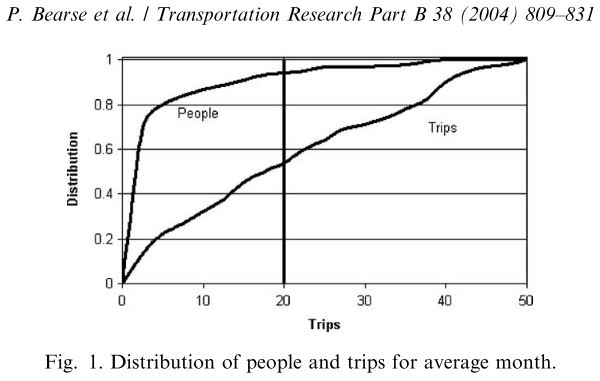
\includegraphics{images/bearse_people_trips_distribution.JPG}
\caption{Distribution of users and number of trips.}
\end{figure}

The Charlottesvill Transit System manages the eligibility process for
Charlottesville users of JAUNT. The figure below shows the growth since
1984 by number of eligible JAUNT users.

\begin{figure}
\centering
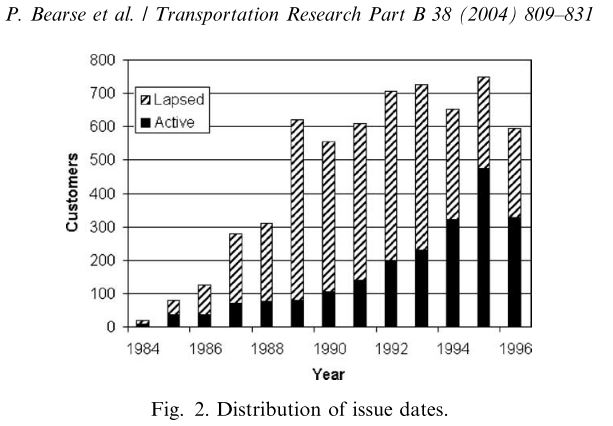
\includegraphics{images/bearse_lapsed_population_growth.JPG}
\caption{Growth of eligibile users.}
\end{figure}

\hypertarget{mobility-as-a-service-and-the-transition-to-driverless-systems}{%
\subsection{Mobility as a Service and the transition to driverless
systems}\label{mobility-as-a-service-and-the-transition-to-driverless-systems}}

\hypertarget{abstract-30}{%
\subsubsection{Abstract}\label{abstract-30}}

From Joschka Bischoff's dissertation, chapter 6 covers wheelchair
accessible taxis.

\hypertarget{assumptions}{%
\subsubsection{Assumptions}\label{assumptions}}

The current paratransit system will be almost completely replaced. WAV
taxis are subsidized instead of using the Special Transit Service (SFD)
in Berlin. 700 daily rides (from the SFD and 10\% WAV) + 300 daily rides
(from tourists, suburban areas, or temporarily disabled individuals) =
1000 assumed daily rides. ``Trips of persons using wheelchairs are
generally similar to non-work trips of persons without disability.''

\hypertarget{methodology}{%
\subsubsection{Methodology}\label{methodology}}

10/100 non-work trips are marked with ``wheelchair-friendly service''.
This is added to the demand in Berlin and matched with taxi/supply
model. Certain vehicles are marked WAV (500-100) aiming to achieve an
average wait time of 15 minutes. The ``nearest vehicle'' with the WAV
requirement is dispatched but not prioritized.

\hypertarget{conclusions}{%
\subsubsection{Conclusions}\label{conclusions}}

With 250 WAV vehicles (well below 5\% of the city's active vehicle
fleet) an estimated wait time of 12:22 minues is acheived.

\end{document}
